\documentclass[tikz,border=10pt]{standalone}
\usepackage{tikz}
\usetikzlibrary{arrows.meta,positioning,fit,backgrounds}

\definecolor{airaBlue}{RGB}{31,78,121}
\definecolor{airaMid}{RGB}{46,117,182}
\definecolor{airaLight}{RGB}{232,240,248}
\definecolor{airaWarn}{RGB}{255,248,232}
\definecolor{airaRed}{RGB}{192,0,0}
\definecolor{airaGray}{RGB}{90,90,90}

\begin{document}
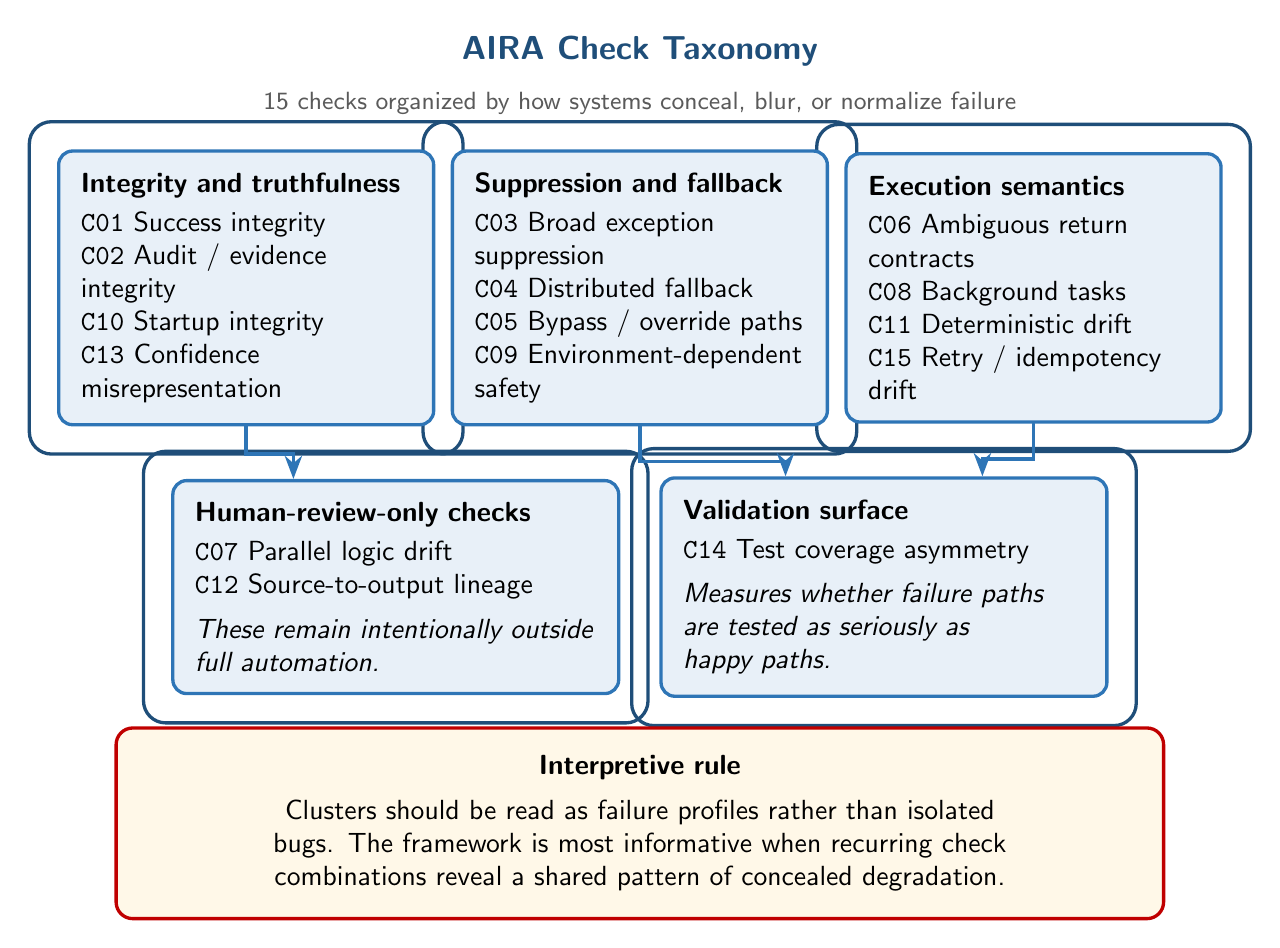
\begin{tikzpicture}[
  font=\sffamily,
  box/.style={rounded corners=5pt, draw=airaMid, fill=airaLight, very thick, align=left, inner sep=8pt, text width=4.2cm},
  cluster/.style={rounded corners=8pt, draw=airaBlue, very thick, inner sep=10pt},
  small/.style={font=\sffamily\small},
  title/.style={font=\sffamily\bfseries\large, text=airaBlue},
  arrow/.style={->, >=Stealth, very thick, draw=airaMid, line cap=round}
]

\node[title] (title) at (0,5.8) {AIRA Check Taxonomy};
\node[small, text=airaGray, align=center] at (0,5.15) {15 checks organized by how systems conceal, blur, or normalize failure};

\node[box] (c01) at (-5.0,2.8) {\textbf{Integrity and truthfulness}\\[2pt]
\texttt{C01} Success integrity\\
\texttt{C02} Audit / evidence\\ integrity\\
\texttt{C10} Startup integrity\\
\texttt{C13} Confidence\\ misrepresentation};

\node[box] (c03) at (0.0,2.8) {\textbf{Suppression and fallback}\\[2pt]
\texttt{C03} Broad exception\\ suppression\\
\texttt{C04} Distributed fallback\\
\texttt{C05} Bypass / override paths\\
\texttt{C09} Environment-dependent\\ safety};

\node[box] (c06) at (5.0,2.8) {\textbf{Execution semantics}\\[2pt]
\texttt{C06} Ambiguous return\\ contracts\\
\texttt{C08} Background tasks\\
\texttt{C11} Deterministic drift\\
\texttt{C15} Retry / idempotency\\ drift};

\node[box, text width=5.1cm] (human) at (-3.1,-1.0) {\textbf{Human-review-only checks}\\[2pt]
\texttt{C07} Parallel logic drift\\
\texttt{C12} Source-to-output lineage\\[4pt]
\emph{These remain intentionally outside\\ full automation.}};

\node[box, text width=5.1cm] (tests) at (3.1,-1.0) {\textbf{Validation surface}\\[2pt]
\texttt{C14} Test coverage asymmetry\\[4pt]
\emph{Measures whether failure paths\\ are tested as seriously as\\ happy paths.}};

\begin{scope}[on background layer]
  \node[cluster, fit=(c01)] {};
  \node[cluster, fit=(c03)] {};
  \node[cluster, fit=(c06)] {};
  \node[cluster, fit=(human)] {};
  \node[cluster, fit=(tests)] {};
\end{scope}

\draw[arrow] (c01.south) -- ++(0,-0.35) -| ([xshift=-1.3cm]human.north);
\draw[arrow] (c03.south) -- ++(0,-0.45) -| ([xshift=-1.25cm]tests.north);
\draw[arrow] (c06.south) -- ++(0,-0.45) -| ([xshift=1.25cm]tests.north);

\node[draw=airaRed, rounded corners=6pt, very thick, fill=airaWarn, inner sep=10pt, text width=12.6cm, align=center] at (0,-4.0) {
\textbf{Interpretive rule}\\[4pt]
Clusters should be read as failure profiles rather than isolated bugs. The framework is most informative when recurring check combinations reveal a shared pattern of concealed degradation.
};
\end{tikzpicture}
\end{document}
